\documentclass[pdftex,12pt,a4paper]{article}

\usepackage{wrapfig,amssymb,amsmath,graphicx, subfigure}
\usepackage[dutch]{babel}
\usepackage[top=0.5in, bottom=0.5in, left=1in, right=1in]{geometry}
\pagenumbering{arabic}
\newcommand{\HRule}{\rule{\linewidth}{0.5mm}}

\begin{document}
\begin{titlepage}

% Upper part of the page
\begin{flushleft}

\includegraphics[trim=23mm 0mm 0mm 0mm, width=1\textwidth]{./logo.jpg}\\[1cm] \end{flushleft}
\begin{center}
	\textsc{\Large Netcentric Computing}\\[0.5cm]

    % Title
    \HRule \\[0.4cm] { \huge \bfseries Report for first week assignment}\\[0.4cm]

    \HRule \\[1.5cm]

    % Author and supervisor
\begin{minipage}{0.4\textwidth}
\begin{flushleft} \large \emph{Authors:}\\
Jaap \textsc{Koetsier}\\
Jelte \textsc{Fennema}\\
Abe \textsc{Wiersma}\\
\end{flushleft}
\end{minipage}
\begin{minipage}{0.4\textwidth} \begin{flushright} \large \end{flushright}\end{minipage}

    \vfill

    % Bottom of the page 
    {\large \today}

\end{center}
\end{titlepage}
\pagebreak
\section{Servo naar Mbed}
De stap van de servo naar de embed ging eigenlijk vrij gemakkelijk, binnen het eerste uur van spelen met de embed software hadden we al uitgevonden hoe de data uitgelezen zou moeten worden. Na een hoop gespeel met voltages kwamen we erachter dat de standen van de potentiometer gekalibreerd zouden moeten worden, van 0 t/m 10 (0.0, 0.005, 0.0215, 0.06, 0.104, 0.149, 0.199, 0.2985, 0.513, 0.76, 0.998).
Bij deze standen bepaalden we ook een precisie opdat de motor stil zou staan op een bepaalde stand, er zit een bepaalde variatie binnen de stilstaande voltage van de potentiometer(0.0005, 0.0005, 0.00075, 0.0015, 0.0025, 0.0025, 0.003, 0.0035, 0.0035, 0.004, 0.001).
Voor interactie met de motor, verbonden aan de mbed, gebruikten we de Hbridge library. Deze library is makkelijk gebruikbaar en van een HBridge object gebruiken we slechts 2 functies, hbridge.power(true). En hbridge.speed([-1.0 - 1.0]) om de richting en snelheid van de motor te bepalen.


\section{Mbed naar Android Telefoon}
\section{Android naar Android}
\section{Conclusie}
\section{Diagram}
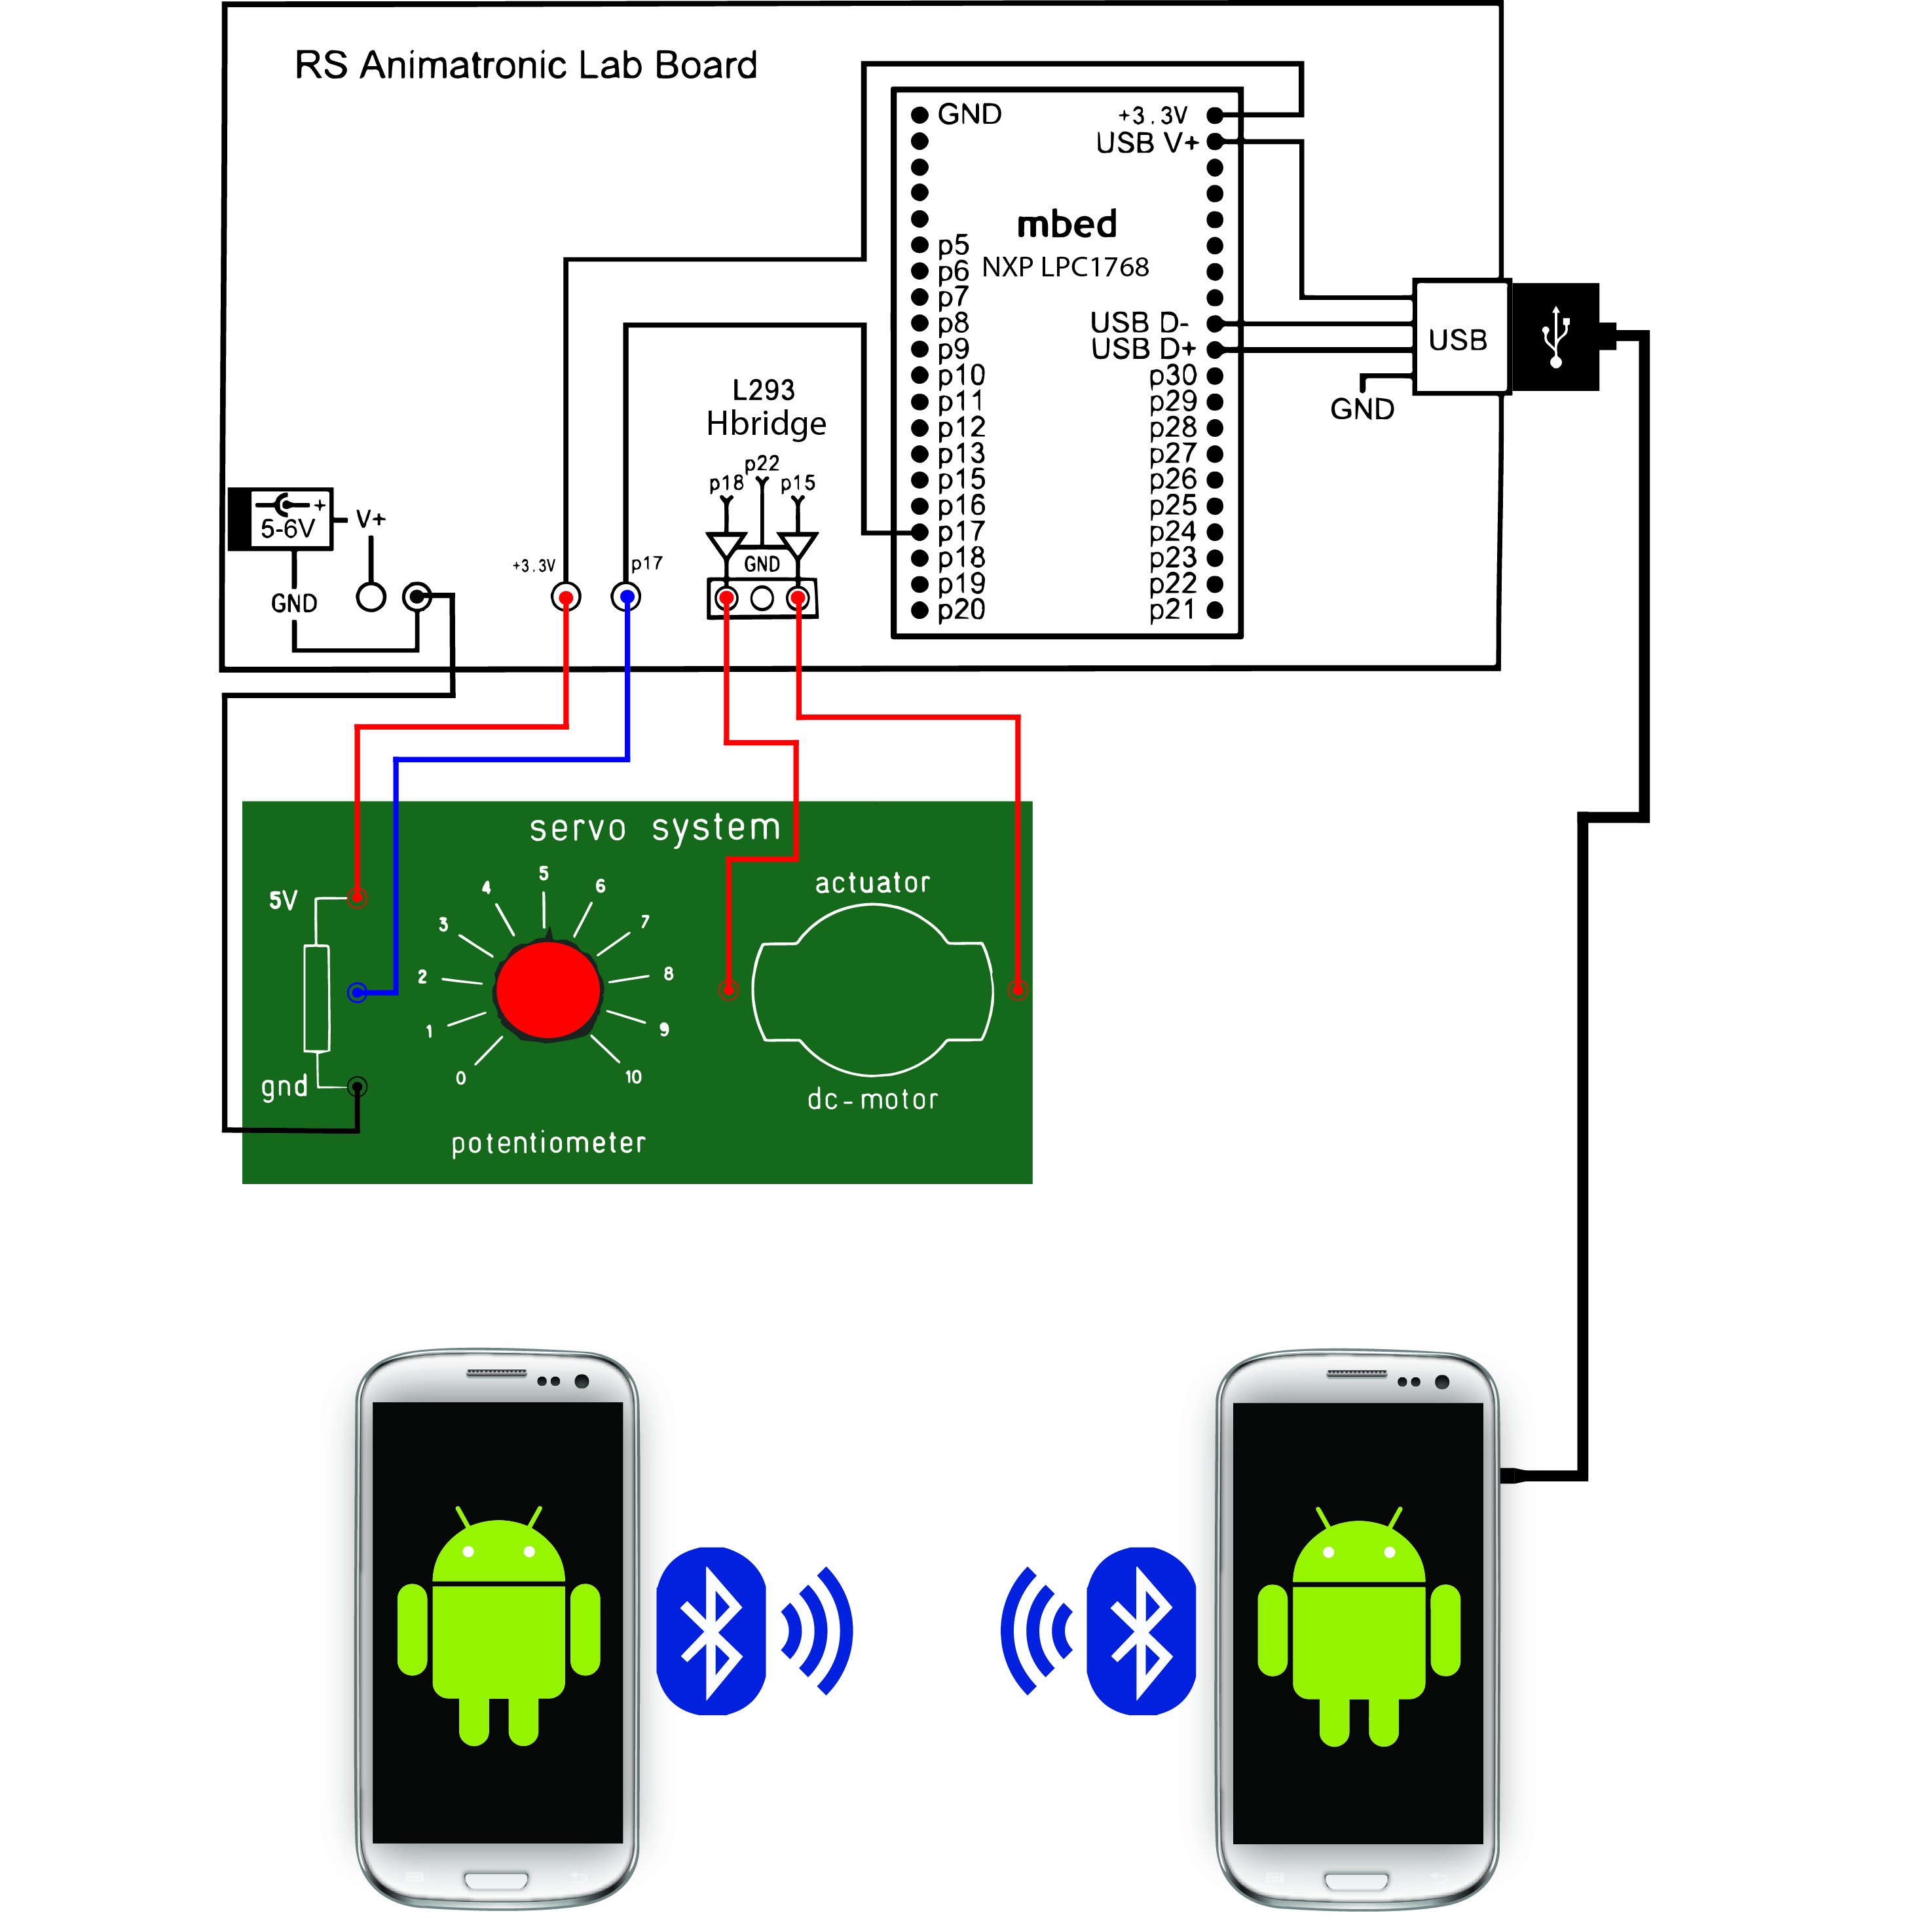
\includegraphics[width=1\textwidth]{./diagram.jpg}\\
\end{document}